%Format: PDF

\documentclass[a4paper,11pt,french]{article}

\addtolength{\textwidth}{10mm}
\addtolength{\oddsidemargin}{-5mm}
\setlength{\parindent}{0mm}
\setlength{\parskip}{.5\baselineskip plus .2\baselineskip
                                     minus .2\baselineskip}

\usepackage{amsmath}
\usepackage{tabvar}
%\usepackage[FlechesPS]{tabvar}
%\usepackage[FlechesMP]{tabvar}

\usepackage[T1]{fontenc}
\usepackage{lmodern}
\usepackage{babel}

\newcommand*{\file}[1]{\texttt{#1}}
\newcommand*{\env}[1]{\texttt{#1}}
\newcommand*{\ctype}[1]{\texttt{#1}}

\begin{document}
\thispagestyle{empty}

\begin{center}
  \Large\bfseries Exemples de tableaux de variations avec \file{tabvar}
\end{center}

Un exemple simple :
$\displaystyle f(x)=\frac{x^3+2}{2x} \qquad f'(x)=\frac{x^3-1}{x^2}$.

\[\begin{tabvar}{|C|CCCCCCCCC|} \hline
 x    &-\infty &   &-\sqrt[3]{2} &   & 0       &   & 1  &    &+\infty
\\ \hline
f'(x) &        & - &             & - & \dbarre & - & 0  & +  &
\\ \hline
\niveau{3}{3}f(x)
      &+\infty                       &\decroit
      &0                             &\decroit
      &\discont{-\infty}{<}{+\infty} &\decroit
      &\frac{3}{2}                   &\croit
      &+\infty
\\ \hline
\end{tabvar}\]

Le codage du tableau est le suivant :
\begin{verbatim}
\[\begin{tabvar}{|C|CCCCCCCCC|} \hline
 x    &-\infty &  &-\sqrt[3]{2} &  &0       &  & 1 &  &+\infty
\\ \hline
f'(x) &        &- &             &- &\dbarre &- & 0 &+ &
\\ \hline
\niveau{3}{3}f(x)
      &+\infty                       &\decroit
      &0                             &\decroit
      &\discont{-\infty}{<}{+\infty} &\decroit
      &\frac{3}{2}                   &\croit
      &+\infty
\\ \hline
\end{tabvar}\]
\end{verbatim}

L'argument optionnel de \verb|\discont| n'a pas été utilisé, on obtiendrait
une meilleure présentation en lui donnant la valeur~1, ce qui écarterait
d'un interligne les valeurs $+\infty$ et~$-\infty$, mettant ainsi
les trois valeurs~$+\infty$ sur la même ligne.

D'autre part, $f(x)$ est placé au niveau~3 par la commande \verb|\niveau|.
Si on souhaite que $f(x)$ soit centré verticalement, on peut utiliser
la commande \verb|\TVcenter|%
\footnote{Cette commande n'est disponible que depuis la version 1.6
  (juillet~2011) de \file{tabvar}.}  :\\
\verb|\niveau{3}{3}\TVcenter{f(x)} &+\infty}|

Voici le résultat obtenu avec ces deux modifications :
\[\begin{tabvar}{|C|CCCCCCCCC|} \hline
 x    &-\infty &  &-\sqrt[3]{2} &  &0       &  & 1 &  &+\infty
\\ \hline
f'(x) &        &- &             &- &\dbarre &- & 0 &+ &
\\ \hline
\niveau{3}{3}\TVcenter{f(x)}
      &+\infty             &\decroit
      &0                                &\decroit
      &\discont[1]{-\infty}{<}{+\infty} &\decroit
      &\frac{3}{2}                      &\croit
      &+\infty
\\ \hline
\end{tabvar}\]

Une présentation plus traditionnelle du tableau de variations serait la
suivante (on renonce à l'utilisation de \verb|\discont| et on remplace
la colonne \ctype{C} par trois colonnes \ctype{LCR}, la colonnne
centrale contenant une double barre).  On ajoute également des filets
verticaux pour les valeurs remarquables de la fonction ou de sa dérivée
grâce à la commande \verb|\barre{}|%
\footnote{Cette commande n'est disponible que depuis la version 1.1 (mai~2007)
  de \file{tabvar}.}
(argument \emph{obligatoire}, éventuellement vide).

\[\begin{tabvar}{|C|CCCCLCRCCCC|} \hline
 x    &-\infty & &-\sqrt[3]{2} & & &0       & & &1         & &+\infty
\\ \hline
f'(x) &        &-& \barre{}    &-& &\dbarre & &-&\barre{0} &+&
\\ \hline
\niveau{3}{3}\TVcenter{f(x)}
      &+\infty                                 &\decroit
      &\barre{0}                               &\decroit
      &-\infty  &\dbarre &\niveau{3}{3}+\infty &\decroit
      &\barre{\frac{3}{2}}                     &\croit
      &+\infty
\\ \hline
\end{tabvar}\]

Le codage est le suivant :
\begin{verbatim}
\[\begin{tabvar}{|C|CCCCLCRCCCC|} \hline
 x   &-\infty& &-\sqrt[3]{2} & & &0       & & &1         & &+\infty
\\ \hline
f'(x)&       &-& \barre{}    &-& &\dbarre & &-&\barre{0} &+&
\\ \hline
\niveau{3}{3}\TVcenter{f(x)}
      &+\infty                                 &\decroit
      &\barre{0}                               &\decroit
      &-\infty  &\dbarre &\niveau{3}{3}+\infty &\decroit
      &\barre{\frac{3}{2}}                     &\croit
      &+\infty
\\ \hline
\end{tabvar}\]
\end{verbatim}

Noter la présence de la seconde commande \verb|\niveau| pour
positionner le terme \verb|+\infty| au niveau~3 après la discontinuité.

\newpage
Un exemple de courbe paramétrée :
$\displaystyle x(t)= t + \frac{1}{t}\qquad y(t) = t + \frac{1}{2t^2}$.

\[
\begin{tabvar}{|C|CCRCCCCCC|} \hline
 t    &-\infty &   &-1  &   & 0       &   & 1  &   &+\infty
\\ \hline
x'(t) &        &+  & 0  & - & \dbarre & - & 0  & + &
\\ \hline
\niveau{1}{3}
\TVcenter{x(t)} &-\infty                          &\croit
                &-2                               &\decroit
                &\discont[1]{-\infty}{<}{+\infty} &\decroit
                &2                                &\croit
                &+\infty
\\ \hline
\niveau{1}{3}
\TVcenter{y(t)} &-\infty        &\croit
                &-\frac{1}{2}   &\croit
                &+\infty        &\decroit
                &\frac{3}{2}    &\croit
                &+\infty
\\ \hline
y'(t) &        &+  &2   & + & \dbarre & - & 0  &+   &
\\ \hline
\end{tabvar}
\]

Le codage est le suivant :
\begin{verbatim}
\[\begin{tabvar}{|C|CCRCCCCCC|} \hline
 t    &-\infty &   &-1  &   & 0       &   & 1  &   &+\infty
\\ \hline
x'(t) &        &+  & 0  & - & \dbarre & - & 0  & + &
\\ \hline
\niveau{1}{3}
\TVcenter{x(t)} &-\infty                          &\croit
                &-2                               &\decroit
                &\discont[1]{-\infty}{<}{+\infty} &\decroit
                &2                                &\croit
                &+\infty
\\ \hline
\niveau{1}{3}
\TVcenter{y(t)} &-\infty        &\croit
                &-\frac{1}{2}   &\croit
                &+\infty        &\decroit
                &\frac{3}{2}    &\croit
                &+\infty
\\ \hline
y'(t) &        &+  &2   & + & \dbarre & - & 0  &+   &
\\ \hline
\end{tabvar}
\]
\end{verbatim}

\newpage
Le même tableau de variations en présentation \og traditionnelle \fg.

\[\begin{tabvar}{|C|CCCCRCLCCCC|} \hline
 t   &-\infty & &-1       & & &0       & & & 1        & &+\infty
\\ \hline
x'(t)&        &+&\barre{0}&-& &\dbarre & &-&\barre{0} &+&
\\ \hline
\niveau{1}{3}
\TVcenter{x(t)} &-\infty                            &\croit
           &\barre{-2}                              &\decroit
           &-\infty  &\dbarre &\niveau{3}{3}+\infty &\decroit
           &\barre{2}                               &\croit
           &+\infty
\\ \hline
\niveau{1}{3}
\TVcenter{y(t)} &-\infty                   &\croit
                &-\frac{1}{2}              &\croit
                &+\infty &\dbarre &+\infty &\decroit
                &\barre{\frac{3}{2}}       &\croit
                &+\infty
\\ \hline
y'(t) &        &+ &2         &+ & &\dbarre & &- &\barre{0} &+ &
\\ \hline
\end{tabvar}\]

Le codage est le suivant :
\begin{verbatim}
\[\begin{tabvar}{|C|CCCCRCLCCCC|} \hline
 t   &-\infty & &-1       & & &0       & & & 1        & &+\infty
\\ \hline
x'(t)&        &+&\barre{0}&-& &\dbarre & &-&\barre{0} &+&
\\ \hline
\niveau{1}{3}
\TVcenter{x(t)} &-\infty                            &\croit
           &\barre{-2}                              &\decroit
           &-\infty  &\dbarre &\niveau{3}{3}+\infty &\decroit
           &\barre{2}                               &\croit
           &+\infty
\\ \hline
\niveau{1}{3}
\TVcenter{y(t)} &-\infty                   &\croit
                &-\frac{1}{2}              &\croit
                &+\infty &\dbarre &+\infty &\decroit
                &\barre{\frac{3}{2}}       &\croit
                &+\infty
\\ \hline
y'(t) &        &+ &2         &+ & &\dbarre & &- &\barre{0} &+ &
\\ \hline
\end{tabvar}\]
\end{verbatim}

Noter que le type de la colonne $t=-1$ a dû être changé de \ctype{R} à
\ctype{C} pour permettre l'ajout du filet vertical.

\newpage
Dans certains cas les filets horizontaux sont placés trop près de certains
éléments du tableau. Ce problème peut être résolu grâce aux extensions
\file{cellspace} ou \file{tabls} mais celles-ci ne fonctionnent pas
avec l’environnement \env{tabvar}. Voici un exemple (fonction
$f(x)=-x^2+x$ sur $[0,1]$) où l’utilisation maladroite de \verb|\dfrac| au
lieu de \verb|\frac| pour coder les fractions $\frac{1}{2}$ et $\frac{1}{4}$
aboutit au tableau de gauche.

\vspace{-.5\baselineskip}
\[\begin{tabvar}{|C|LCCCR|}
\hline
x                            &0            &       &\dfrac{1}{2} &         & 1
\\ \hline
f'(x)                        &1\phantom{-} & +     & 0           & -       &-1
\\ \hline
\niveau{1}{2}\TVcenter{f(x)} &0            &\croit &\dfrac{1}{4} &\decroit & 0
\\ \hline
\end{tabvar}
\quad
\begin{tabvar}{|C|LCCCR|}
\hline
x                            &0 &       &\TVstretch{\dfrac{1}{2}} &         & 1
\\ \hline
f'(x)                        &1\phantom{-} & +     & 0            & -       &-1
\\ \hline
\niveau{1}{2}\TVcenter{f(x)} &0 &\croit &\TVstretch{\dfrac{1}{4}} &\decroit & 0
\\ \hline
\end{tabvar}\]

\vspace{-.3\baselineskip}
Le codage du tableau de gauche est le suivant :
\vspace{-.2\baselineskip}
{\footnotesize
\begin{verbatim}
\begin{tabvar}{|C|CCCCR|}
\hline
x                            &0            &       &\dfrac{1}{2} &         & 1
\\ \hline
f'(x)                        &1\phantom{-} & +     & 0           & -       &-1
\\ \hline
\niveau{1}{2}\TVcenter{f(x)} &0            &\croit &\dfrac{1}{4} &\decroit & 0
\\ \hline
\end{tabvar}
\end{verbatim}
}

\vspace{-.3\baselineskip}
Le tableau de droite est obtenu grâce à la commande \verb|\TVstretch|%
\footnote{Cette commande n'est disponible que depuis la version 1.7
  (décembre~2012) de \file{tabvar}.} ;
il suffit de remplacer \verb|\dfrac{1}{2}| et \verb|\dfrac{1}{4}|
par \verb|\TVstretch{\dfrac{1}{2}}| et \verb|\TVstretch{\dfrac{1}{4}}| ce qui
ajoute un petit espace vertical (\verb|2pt| soit 0,6mm environ) au-dessus et
au-dessous de ces fractions.

La commande \verb|\TVstretch| peut aussi s’utiliser avec un argument
optionnel qui ajoute de l’espace uniquement au-dessus ou au-dessous selon son
signe. Le codage\par
\vspace{-.3\baselineskip}
{\footnotesize
\begin{verbatim}
\begin{tabvar}{|C|R C C C C|}
\hline
x    &0 &      &\TVstretch[-4pt]{\frac{1}{2}} &        & 1
\\ \hline
f'(x)&-1 & -    & 0                    & +      &1
\\ \hline
\niveau{2}{2}\TVcenter{f(x)} &\TVstretch[2pt]{1} &\decroit&\frac{1}{4} &\croit&1
\\ \hline
\end{tabvar}
\end{verbatim}
}

\enlargethispage*{1.1\baselineskip}
\vspace{-.3\baselineskip}
produit le tableau de droite, le tableau de gauche est obtenu avec le même
codage mais sans recours à la commande \verb|\TVstretch|.
\[\begin{tabvar}{|C|R C C C C|}
\hline
x    &0  &      &\frac{1}{2} &        & 1
\\ \hline
f'(x)&-1 & -    & 0                    & +      &1
\\ \hline
\niveau{2}{2}\TVcenter{f(x)} &1 &\decroit&\frac{1}{4} &\croit&1
\\ \hline
\end{tabvar}
\quad
\begin{tabvar}{|C|R C C C C|}
\hline
x    &0  &      &\TVstretch[-4pt]{\frac{1}{2}} &        & 1
\\ \hline
f'(x)&-1 & -    & 0                    & +      &1
\\ \hline
\niveau{2}{2}\TVcenter{f(x)} &\TVstretch[2pt]{1} &\decroit&\frac{1}{4} &\croit&1
\\ \hline
\end{tabvar}
\]


\newpage
Il est possible de choisir entre quatre types de flèches grâce aux commandes
\verb+\FlechesPS1+ (flèches « à moustaches » obtenues par défaut) \dots{}
\verb+\FlechesPS4+.
Voici le même tableau avec des flèches assorties à la police Fourier
(\verb+\FlechesPS2+) :

\FlechesPS2
\[\begin{tabvar}{|C|CCCCRCLCCCC|} \hline
 t    &-\infty &  &-1        &  & &0       & &  & 1        &  &+\infty
\\ \hline
x'(t) &        &+ &\barre{0}
                             &- & &\dbarre & &- &\barre{0} &+ &
\\ \hline
\niveau{1}{3}
\TVcenter{x(t)} &-\infty                                 &\croit
                &\barre{-2}                              &\decroit
                &-\infty  &\dbarre &\niveau{3}{3}+\infty &\decroit
                &\barre{2}                               &\croit
                &+\infty
\\ \hline
\niveau{1}{3}
\TVcenter{y(t)} &-\infty                         &\croit
                &-\frac{1}{2}              &\croit
                &+\infty &\dbarre &+\infty &\decroit
                &\barre{\frac{3}{2}}       &\croit
                &+\infty
\\ \hline
y'(t) &        &+ &2         &+ & &\dbarre & &- &\barre{0} &+ &
\\ \hline
\end{tabvar}\]

Une autre variante (\verb+\FlechesPS3+) \FlechesPS3 :
\[\begin{tabvar}{|C|CCCCRCLCCCC|} \hline
 t    &-\infty &  &-1        &  & &0       & &  & 1        &  &+\infty
\\ \hline
x'(t) &        &+ &\barre{0}
                             &- & &\dbarre & &- &\barre{0} &+ &
\\ \hline
\niveau{1}{3}
\TVcenter{x(t)} &-\infty                                 &\croit
                &\barre{-2}                              &\decroit
                &-\infty  &\dbarre &\niveau{3}{3}+\infty &\decroit
                &\barre{2}                               &\croit
                &+\infty
\\ \hline
\niveau{1}{3}
\TVcenter{y(t)} &-\infty                         &\croit
                &-\frac{1}{2}              &\croit
                &+\infty &\dbarre &+\infty &\decroit
                &\barre{\frac{3}{2}}       &\croit
                &+\infty
\\ \hline
y'(t) &        &+ &2         &+ & &\dbarre & &- &\barre{0} &+ &
\\ \hline
\end{tabvar}\]

et une dernière (\verb+\FlechesPS4+) \FlechesPS4 :
\[\begin{tabvar}{|C|CCCCRCLCCCC|} \hline
 t    &-\infty &  &-1        &  & &0       & &  & 1        &  &+\infty
\\ \hline
x'(t) &        &+ &\barre{0}
                             &- & &\dbarre & &- &\barre{0} &+ &
\\ \hline
\niveau{1}{3}
\TVcenter{x(t)} &-\infty                                 &\croit
                &\barre{-2}                              &\decroit
                &-\infty  &\dbarre &\niveau{3}{3}+\infty &\decroit
                &\barre{2}                               &\croit
                &+\infty
\\ \hline
\niveau{1}{3}
\TVcenter{y(t)} &-\infty                         &\croit
                &-\frac{1}{2}              &\croit
                &+\infty &\dbarre &+\infty &\decroit
                &\barre{\frac{3}{2}}       &\croit
                &+\infty
\\ \hline
y'(t) &        &+ &2         &+ & &\dbarre & &- &\barre{0} &+ &
\\ \hline
\end{tabvar}\]

\newpage

Enfin il est possible d'élargir les colonnes contenant des flèches grâce à la
commande \verb|\TVarrowscolstretch| ou d'ajouter de l'espace entre les
colonnes avec \verb|\TVarraycolsep|, voici le même tableau composé avec

{\verb|\renewcommand*{\TVarrowscolstretch}{1.2}|\quad (1.0 par défaut)\\
\verb|\setlength{\TVarraycolsep}{5pt}|\quad (1pt par défaut)
\renewcommand*{\TVarrowscolstretch}{1.2}
\setlength{\TVarraycolsep}{5pt}
\FlechesPS3
\[\begin{tabvar}{|C|CCCCRCLCCCC|} \hline
 t    &-\infty &  &-1        &  & &0       & &  & 1        &  &+\infty
\\ \hline
x'(t) &        &+ &\barre{0}
                             &- & &\dbarre & &- &\barre{0} &+ &
\\ \hline
\niveau{1}{3}
\TVcenter{x(t)} &-\infty                                 &\croit
                &\barre{-2}                              &\decroit
                &-\infty  &\dbarre &\niveau{3}{3}+\infty &\decroit
                &\barre{2}                               &\croit
                &+\infty
\\ \hline
\niveau{1}{3}
\TVcenter{y(t)} &-\infty                         &\croit
                &-\frac{1}{2}              &\croit
                &+\infty &\dbarre &+\infty &\decroit
                &\barre{\frac{3}{2}}       &\croit
                &+\infty
\\ \hline
y'(t) &        &+ &2         &+ & &\dbarre & &- &\barre{0} &+ &
\\ \hline
\end{tabvar}\]
}

D'autres possibilités d'ajustements existent, consulter le fichier
\file{tabvar.cfg}.

Le même tableau encore, mais cette fois on utilise les flèches dessinées en
MetaPost. Celles-ci sont conservées uniquement pour préserver la compatibilité
ascendante, l'utilisation des flèches PostScript est de loin préférable (les
flèches MetaPost sont des \emph{dessins}, leur couleur ne change pas avec la
couleur du texte contrairement aux flèches PostScript qui sont des
\emph{caractères}).
Les flèches MetaPost sont obtenues avec
\verb|\usepackage[FlechesMP]{tabvar}|
ou la commande \verb|\FlechesMPtrue| placée dans le préambule ou dans le
fichier \file{tabvar.cfg}.

\begingroup
  \newsavebox{\arup}%
  \newsavebox{\ardown}%
  \newsavebox{\arhor}%
  \sbox{\arup}{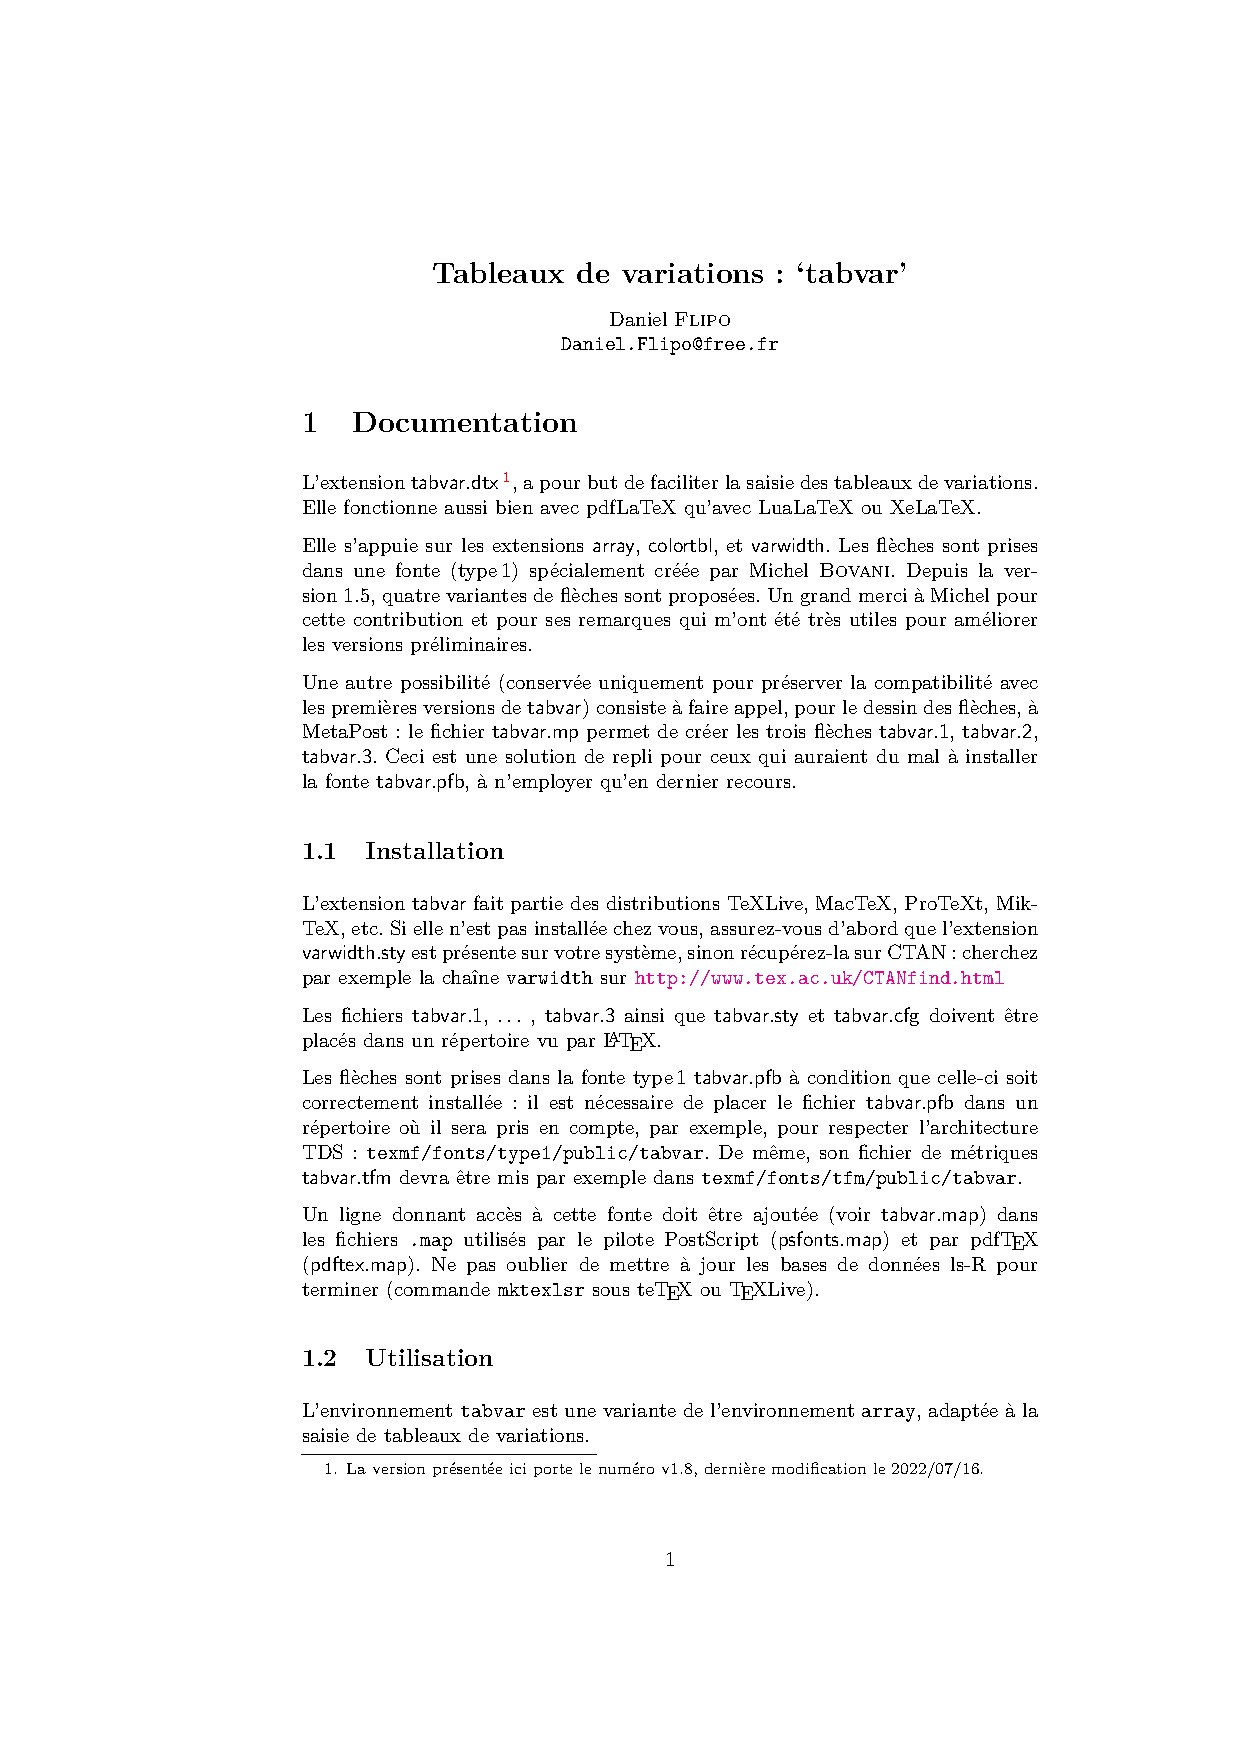
\includegraphics[scale=\TVarrowscale]{tabvar.1}}%
  \sbox{\ardown}{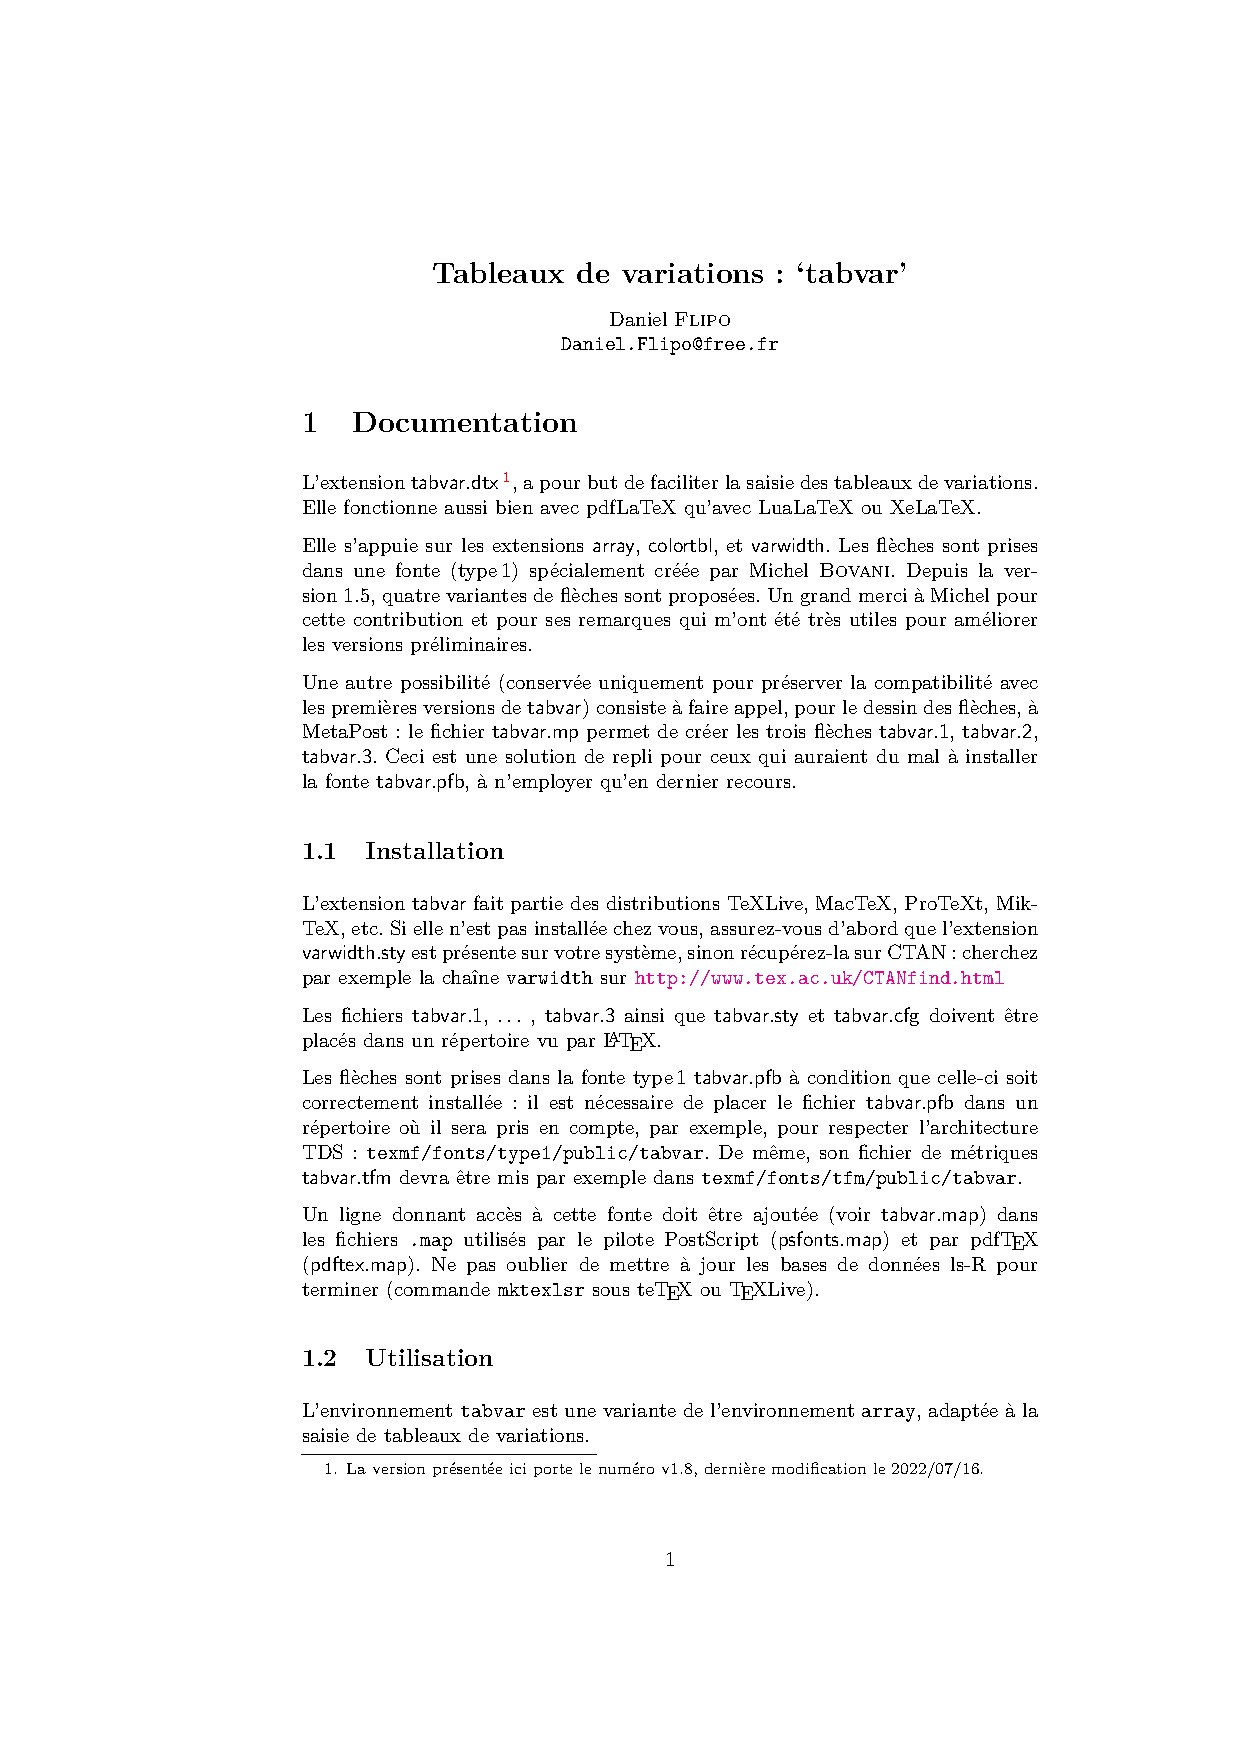
\includegraphics[scale=\TVarrowscale]{tabvar.2}}%
  \sbox{\arhor}{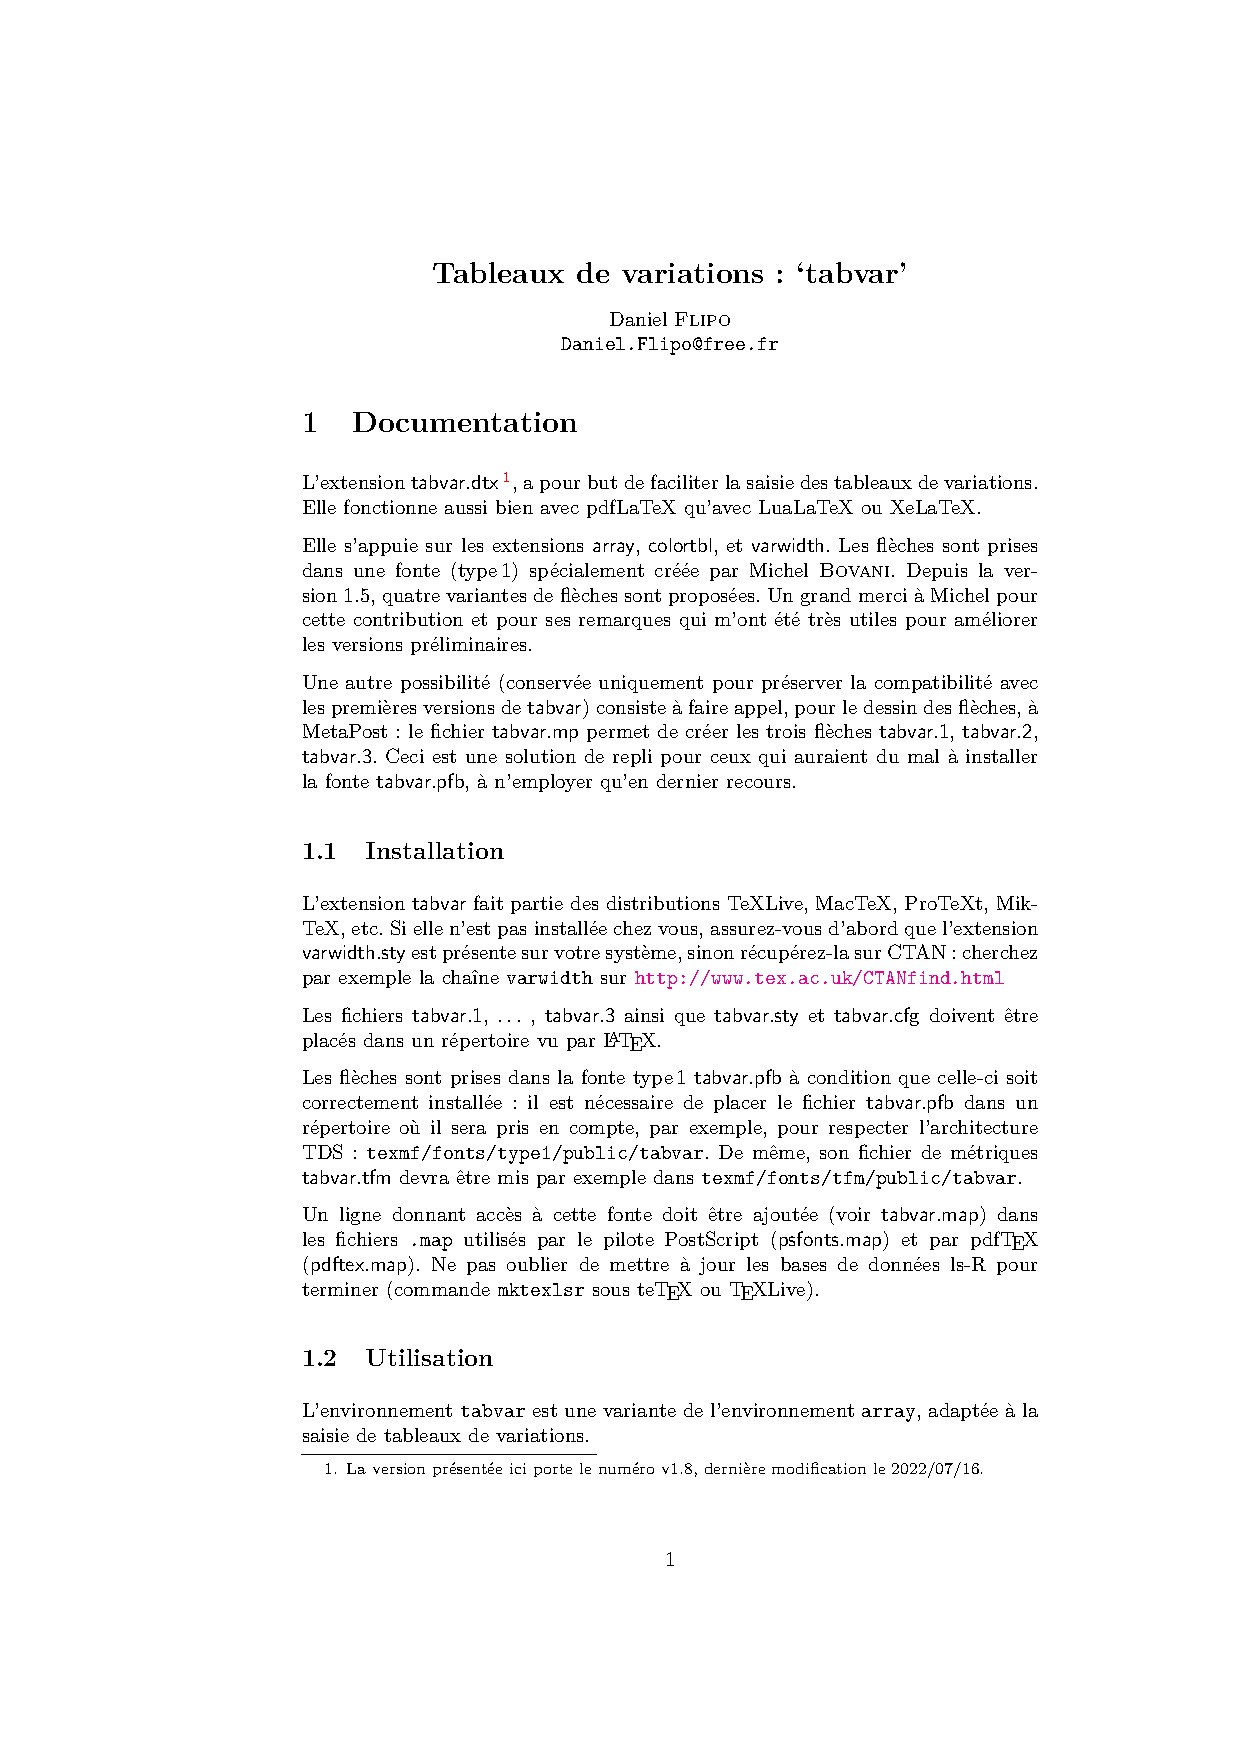
\includegraphics[scale=\TVarrowscale]{tabvar.3}}%
  \makeatletter
  \renewcommand{\FlecheC}{%
        \TV@arrowcol@stretch{\raisebox{.5ex}{\usebox{\arup}}}}%
  \renewcommand{\FlecheD}{%
        \TV@arrowcol@stretch{\raisebox{.5ex}{\usebox{\ardown}}}}%
  \renewcommand{\FlecheH}{%
        \TV@arrowcol@stretch{\raisebox{.5ex}{\usebox{\arhor}}}}%
  \makeatother

  \[\begin{tabvar}{|C|CCCCRCLCCCC|} \hline
   t    &-\infty &  &-1        &  & &0       & &  & 1        &  &+\infty
  \\ \hline
  x'(t) &        &+ &\barre{0}
                               &- & &\dbarre & &- &\barre{0} &+ &
  \\ \hline
  \niveau{1}{3}
  \TVcenter{x(t)} &-\infty                                 &\croit
                  &\barre{-2}                              &\decroit
                  &-\infty  &\dbarre &\niveau{3}{3}+\infty &\decroit
                  &\barre{2}                               &\croit
                  &+\infty
  \\ \hline
  \niveau{1}{3}
  \TVcenter{y(t)} &-\infty                         &\croit
                  &-\frac{1}{2}              &\croit
                  &+\infty &\dbarre &+\infty &\decroit
                  &\barre{\frac{3}{2}}       &\croit
                  &+\infty
  \\ \hline
  y'(t) &        &+ &2         &+ & &\dbarre & &- &\barre{0} &+ &
  \\ \hline
  \end{tabvar}\]
\endgroup

\newpage
\FlechesPS2
Un exemple de fonction non définie partout :
$\displaystyle f(x) = \sqrt{\frac{x-1}{x+1}}$.

\[\begin{tabvar}{|C|CCRULCC|} \hline
 x     &-\infty &  &-1 &\hspace*{15mm} & 1      &  &+\infty
\\ \hline
 f'(x) &        &+ &   &               &+\infty &+ &
\\ \hline
\niveau{1}{2}
\TVcenter{f(x)}&1     &\croit &+\infty   &
          &\niveau{1}{2}0 &\croit & 1
\\ \hline
\end{tabvar}\]

Le codage est le suivant :

\vspace{-.3\baselineskip}
{\footnotesize
\begin{verbatim}
\[\begin{tabvar}{|C|CCRULCC|} \hline
 x     &-\infty &  &-1 &\hspace*{15mm} & 1      &  &+\infty
\\ \hline
 f'(x) &        &+ &   &               &+\infty &+ &
\\ \hline
\niveau{1}{2}
\TVcenter{f(x)}&1     &\croit &+\infty   &
          &\niveau{1}{2}0 &\croit & 1
\\ \hline
\end{tabvar}\]
\end{verbatim}
}

\vspace{-.3\baselineskip}
La largeur de la colonne grisée est fixée à~15mm par le \verb|\hspace*{15mm}|
placé dans une ligne quelconque du tableau. Certains visualiseurs
(Xdvi par exemple) n'affichent pas correctement les couleurs ;
en cas de doute, vérifier sur une sortie PostScript ou PDF.

Noter l'emploi d'une seconde commande \verb|\niveau{1}{2}| pour positionner
la valeur de~$f$ au point~1 (sans celle-ci, cette valeur serait placée
au niveau de la valeur précédente, ici~$+\infty$.

Si on prolongeait la définition de $f$ en posant $f(x)=0$ sur $[-1,1]$
on aurait le tableau suivant :

\vspace{-.3\baselineskip}
\[\begin{tabvar}{|C|CCRCCCCC|} \hline
 x     &-\infty &  &  &-1      &   & 1      &  &+\infty
\\ \hline
 f'(x) &        &+ &  &\dbarre & 0 &+\infty &+ &
\\ \hline
\niveau{1}{2}
\TVcenter{f(x)}  &1        &\croit &+\infty &\niveau{1}{2}0
                                   &\constante &0 &\croit & 1
\\ \hline
\end{tabvar}\]

\enlargethispage*{.5\baselineskip}
Le codage est le suivant :
\vspace{-.3\baselineskip}
{\footnotesize
\begin{verbatim}
\[\begin{tabvar}{|C|CCRCCCCC|} \hline
 x     &-\infty &  &  &-1      &   & 1      &  &+\infty
\\ \hline
 f'(x) &        &+ &  &\dbarre & 0 &+\infty &+ &
\\ \hline
\niveau{1}{2}
\TVcenter{f(x)}  &1        &\croit &+\infty &\niveau{1}{2}0
                                   &\constante &0 &\croit & 1
\\ \hline
\end{tabvar}\]
\end{verbatim}
}
\end{document}

%%% Local Variables:
%%% mode: latex
%%% TeX-master: t
%%% coding: utf-8
%%% End:
